\section{The Web}

\subsection{Basic structure}

The \textit{World Wide Web}, or more commonly \textit{Web}, is a collection of documents and other resources
that can be shared among various devices via the \textit{Internet}.

The resources shared are usually in the form of \textit{web pages}, documents whose structure is defined with HTML
(\textit{Hypertext Markup Language}) and whose styles are declared with CSS (\textit{Cascade Style Sheet}).
Other kind of resources include anything ranging from images, videos, audio, software, and source code.

However, web pages are \textit{static} if they only use HTML and CSS, and cannot do much aside from showing content. A programming
language is hence needed to make the web \textit{dynamic}. Among all technologies and languages, nowadays
only JavaScript survives as the de facto standard language, used for both simple scripts and complex applications.

\subsection{JavaScript}
\label{sec:introduction-javascript}

\textit{JavaScript}, or \textit{JS} when abbreviated, is a high-level, dynamic, weakly typed programming language
that together with HTML and CSS is at the core of the World Wide Web. It conforms to the ECMAScript standard \cite{ecma-262}
and it can be both interpreted and \textit{just-in-time compiled}.
A notable language which is a superset of JavaScript is \textit{TypeScript}, developed by Microsoft, that
introduces static typing and can be transpiled to JavaScript.

\begin{code}[language=javascript, caption=A simple example of JavaScript]
function fact(n) {
  if (n == 0) return 1;
  return n * fact(n - 1);
}

function showFactorial() {
  let div = document.getElementById('output');
  let input = document.getElementById('number');
  let n = parseInt(input.text);

  if (n < 0) {
    div.innerHTML = 'Not defined';
  } else {
    div.innerHTML = fact(n);
  }
}

document
  .getElementById('get-factorial')
  .addEventListener('click', showFactorial)
\end{code}

However, JavaScript is ill-equipped when it comes to performance-critical modern web
pages - from this needs were born technologies such as \textit{asm.js}, \textit{Native Client}, and eventually \textit{WebAssembly}.
The main downsides of JavaScript that brought the need for WebAssembly are:
\begin{itemize}
  \item JavaScript is \textit{always} represented as a text format, so it must be parsed by the user's browser for it to be compiled and enhanced;
  \item JavaScript is dynamically typed, hence optimisations for JS (when possible) have to occur
        in the browser, when all JS files have been received;
        for example, JS has only two numeric type (a double-precision IEEE 754 value and a \textit{BigInt}
        for numbers bigger than $2^{53}$) and this restricts the usable CPU instructions;
  \item JavaScript has a number of security vulnerabilities that WebAssembly strives to eliminate by design;
        a common security vulnerability\footnote{Software vulnerabilities are the most common, but hardware vulnerabilities have also been found \cite{spectre}.}
        in the JavaScript world is \textit{cross-site scripting} (XSS), which is a violation of the
        same-origin policy and occurs when an attacker is able to inject a malicious script in a target website;
        another vulnerability is \textit{cross-site request forgery} (CSRF), in which malicious code on an attacker's website
        tricks the user's browser, so that it takes actions not desired by the user.
\end{itemize}

\subsection{Web browsers and JavaScript runtimes}

A \textit{web browser} is a piece of software for accessing web pages shared on the World Wide Web, or a
local website. Browsers natively support the rendering of HTML and CSS, and feature an engine able to run JavaScript or, more commonly,
to just-in-time compile it in order to improve performance.

Browsers can also mitigate the risk provided by the common JavaScript vulnerabilities mentioned in Section \ref{sec:introduction-javascript}
by using two main methods - \textit{sandboxing}, so that JS isn't allowed to perform general-purpose
programming tasks like working directly with files\footnote{Although, there are APIs that can grant access to a ``virtual drive''
only when explicitly allowed by the user \cite{filesystem-mdn}, so access to the user's file system is not possible.},
and \textit{same-origin policy} constraints, in which scripts from one website have access to data from the same website but not from others.

JavaScript can not only be executed on a browser, but also on so called ``back-end''
runtimes\footnote{Opposed to ``front-end'', which usually pertains to the browser.}.
These runtimes offer custom libraries that permit JavaScript to access the file system, to make network requests,
spawn child processes and build complex applications, for example web servers.
Two notable open-source runtimes are \textit{Node.js}\footnote{\url{https://nodejs.org/}} and \textit{Deno}\footnote{\url{https://deno.land}},
both built on top of Google's V8 engine.
The first is older, initially released in 2009, and has a package manager called \textit{npm}
in order to manage its vast ecosystem of JS packages.
Deno, on the other hand, is a more modern runtime written in Rust, includes support for TypeScript out of the box
and is \textit{secure by default} since it blocks all file, network, and environment access unless explicitly enabled.

\section{WebAssembly}

\subsection{Description and motivations}

\textit{WebAssembly} \cite{wasm-website} is a binary instruction format for a stack-based virtual machine.
It is designed to be a portable compilation target, so that different languages can be deployed on the web.
It was announced in 2015 and implemented by major browsers by 2017, and as of May 2022 is supported
by 93\% of all browsers \cite{caniuse, webassembly-mdn}.
WebAssembly main goals are the following \cite{bringing-the-web-up-to-speed-2017}:
\begin{itemize}
  \item \textit{security}, since code on the Web originates from untrusted sources;
  \item \textit{speed}, by using ahead-of-time optimisations in a similar manner as native machine code;
  \item \textit{portability}, since the web spans many devices, architectures, operating systems, and browsers;
  \item and finally \textit{compactness}, because code is transmitted over the network and must reduce load times as much as possible.
\end{itemize}

There were previous attempt at solving the problem of having safe, fast, and portable low-level code on the Web,
such as \textit{ActiveX}, \textit{Native Client}, and \textit{asm.js}.

\textit{ActiveX} \cite{activex} was a Microsoft's technology for code-signing x86 binaries to run on the web, and relied only
on this signing. Hence, it achieved security through a trust model instead of technical construction.
\textit{Native Client} \cite{native-client} introduced the first sandboxing technique for x86, ARM or MIPS machine code,
which was statically validated. Lastly, \textit{asm.js} \cite{asmjs} is a specialised subset of JavaScript, which is one of the target
languages of \textit{Emscripten} \cite{emscripten}, a compiler toolchain able to compile C/C++ applications in order to have them
run on browsers or on other JavaScript runtimes.

WebAssembly is available as a target for various languages, such as C/C++ with the aid of Emscripten, Rust,
AssemblyScript\footnote{A language with a syntax similar to TypeScript.}, Go, Kotlin, Swift, and Zig.
The compiled binary can be then used from JavaScript on the web, or with Node.js or Deno, or even as a CLI application
with the aid of \textit{WebAssembly runtimes} and the \textit{WebAssembly System Interface}
for accessing system resources (see Section \ref*{sec:introduction-wasi}).

WebAssembly resolves many of the problems of JavaScript, the major ones being:
\begin{itemize}
  \item being represented with a \textit{binary} format, parsing on the client is faster and simpler;
  \item having a static type systems, optimisations can be done earlier at compile time, and not on the browser once all the files
        have already been transferred;
\end{itemize}

\subsection{Overview of the language}

Although WebAssembly is a binary code format, it can also be written with \textit{S-expressions}
in order to be more readable.
Each binary takes the form of a \textit{module}, which contains \textit{functions}, \textit{global} variables,
\textit{tables}, and \textit{memories}. Each of these can be exported to be used in the embedder, and a module can also import functionalities.
While a module is a static representation of a program, an \textit{instance} is the dynamic one.
A module can be instantiated by the embedder (e.g., a JavaScript virtual machine).

\begin{code}[language=wasm, caption={Recursive factorial written in WebAssembly S-expressions}, label=lst:wasm-fact]
  (module
    (func $fact (param $x i64) (result i64)
      (if (result i64) (i64.eqz (local.get $x))
        (then (i64.const 1))
        (else
          (i64.mul
            (local.get $x)
            (call $fact
              (i64.sub (local.get $x) (i64.const 1)))))))
    (export "fact" (func $fact)))
\end{code}

WebAssembly is a typed language, but there are only four basic \textit{value types} - integers and IEEE 754 floating
point numbers, each in 32 and 64 bit variants. There are no distinction between signed and unsigned integers,
but instructions that depends on the present of the sign are marked with an explicit suffix.

\textit{Functions} are typed, take a sequence of values as a parameter, and returns another sequence of values.
They cannot be nested inside each other. The content of the call stack for execution are separate from the data
portion of the memory, and cannot be accessed directly by WebAssembly.
The code inside a function consists of a series of \textit{instructions} that modify an implicit operand stack,
either by declaring local variables or applying operations to the value already on the stack.
Functions can be called either \textit{directly} by using an index that identifies a function, or \textit{indirectly},
i.e., dynamically through a global \textit{table} as shown in Figure \ref{fig:indirect-function-table-structure}.
In this second case, only the function's type signature is validated.

\begin{figure}[h]
  \centering
  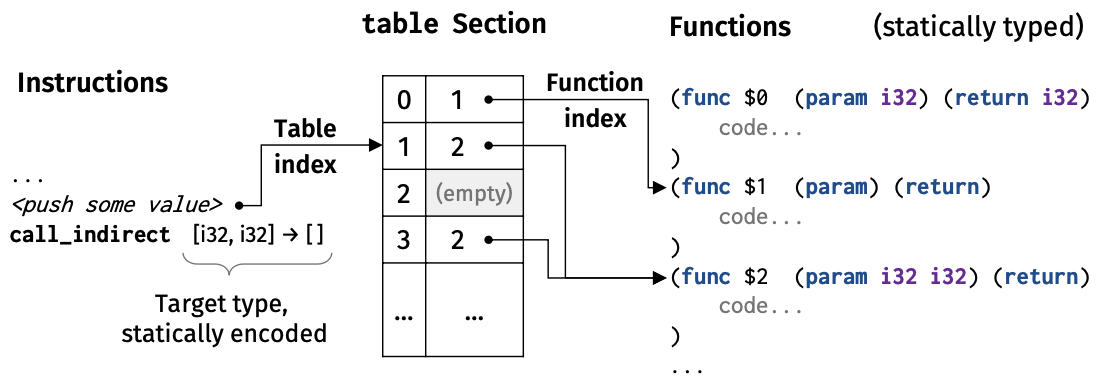
\includegraphics[width=0.8\linewidth]{wasm-function-table.png}
  \caption{The structure of the indirect functions table, from \cite{binary-security-wasm-2020}.}
  \label{fig:indirect-function-table-structure}
\end{figure}

WebAssembly has also support for \textit{traps} - in a similar manner to an exception, a trap aborts the current
computation, and control is given back to the embedder. For example, when embedded in JavaScript, a trap will
throw a JavaScript exception.

The main memory layout that WebAssembly uses is a \textit{linear memory} (or simply \textit{memory}) represented
by an array of bytes. A \textit{linear memory} is a simple addressing technique in which memory appears to the
program as a single contiguous access space \cite{processor-microarchitecture}, which the CPU can access both directly as well as linearly
without resorting to memory segmentation or pagination schemes, enhancing flexibility and reducing latency.
Each module can define no more than one memory, which can grow by one or more
\textit{pages}\footnote{A page is 64 KiB large.} if the need arises.
Access to the individual locations is done through addresses, represented as unsigned integers,
which are dynamically checked against memory size\footnote{On 64 bit platforms the WebAssembly engine
can make use of virtual memory techniques to eliminate this checks, see \cite{bringing-the-web-up-to-speed-2017}.}
(out of bounds accesses result in a trap).
Linear memory also brings security benefits - it is disjoint from the code space, the execution stack and the engine's
data structures \cite{bringing-the-web-up-to-speed-2017}; hence, compiled program cannot corrupt directly their own execution
environment or perform undefined behaviour.

Lastly, WebAssembly doesn't provide arbitrary jumps but \textit{structured control flow},
so that the code can be validated in a single pass and prevent common control flow attacks.

\subsection{Problems with WebAssembly}

Since languages with manual memory management, such as C/C++, can be compiled into WebAssembly,
it is natural to ponder how memory vulnerabilities affect WebAssembly binaries.
In the original paper it is mentioned that ``a buggy or exploited WebAssembly program can make a mess of the data in its own memory''
\cite{bringing-the-web-up-to-speed-2017}, in light of the fact that the call stack is not accessible by the program.

However, even though WebAssembly strives for security, binaries can be still exploited with both traditional attacks,
such as buffer overflows, and attacks that aren't applicable in traditional native binaries, e.g., overwriting
string literals in memory \cite{binary-security-wasm-2020}.

The paper shows that it is possible to obtain a write primitive given a WebAssembly binary compiled from vulnerable C/C++ code,
by means of stack-based buffer overflows and heap metadata corruption, and it is possible to overwrite stack, heap, and ``constant''
data, since the linear memory does not have a read-only section. It would be possible then, for example, to overwrite the name
of a file that was encoded as a string literal in the original program.

Another problem shown in the same paper is the redirection of indirect calls. Since WebAssembly allows indirect calls
to functions through a function table, an attacker could divert the execution by overwriting an integer in linear memory
that serves as an index into the table section. WebAssembly limits this ability with two mechanisms - not all functions
may appear in the table, but only those that can be indirectly called, and all functions call are type checked.
So, redirecting indirect calls is possible only within the class of functions with the same type.

Lastly, it is possible to enable remote code execution when including vulnerable WebAssembly in an application.
This is because functions that have different types in one language can be mapped onto functions with the same type
in WebAssembly. For example, a log function that in C has the signature \texttt{void log(int)}, and a function such as
\texttt{void exec(const char* cmd)} both become functions with only one \texttt{i32} param in WebAssembly.
This enables the indirect diversion described in the previous paragraph if the two functions can be indirectly called.

\subsection{WASI - WebAssembly System Interface}
\label{sec:introduction-wasi}

The \textit{WebAssembly System Interface} (WASI) \cite{wasi} is a modular system interface for WebAssembly.
It focuses on security and portability so that WebAssembly binaries can be targeted by different languages
and then be safely run on different platforms.
Its API provides access to several OS-like features, such as file systems and Berkeley sockets.
The two languages that have good interoperability at the moment are Rust, where the compiler directly supports targeting both WASM and WASI,
and C/C++, either through Emscripten or a custom prebuilt \textit{Clang} toolchain\footnote{\url{https://github.com/WebAssembly/wasi-sdk}}.
These compilers can produce very different memory layouts, as visible in Figure \ref{fig:different-wasm-memory-layouts}.

\begin{figure}[h]
  \centering
  \begin{subfigure}[b]{0.4\textwidth}
    \centering
    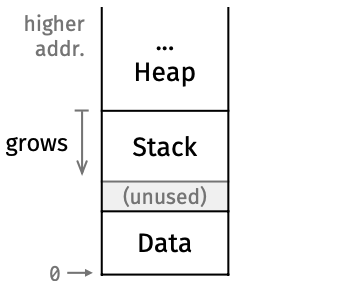
\includegraphics[width=\textwidth]{wasm-memory-emcc-clang9.png}
    \caption{Emscripten 1.39.7, Clang 9\\(without \texttt{stack-first}).}
  \end{subfigure}
  \begin{subfigure}[b]{0.4\textwidth}
    \centering
    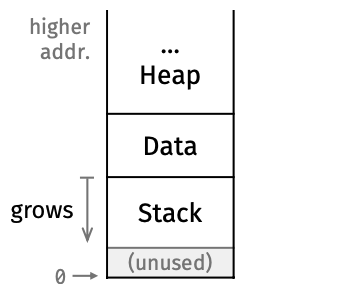
\includegraphics[width=\textwidth]{wasm-memory-clang9-rustc.png}
    \caption{Clang 9 (with \texttt{stack-first}), Rust 1.41 (WASI target).}
  \end{subfigure}
  \caption{Examples of WebAssembly memory layouts obtained from different compilers, from \cite{binary-security-wasm-2020}.}
  \label{fig:different-wasm-memory-layouts}
\end{figure}

A binary that uses WASI can be run using a CLI runtime, such as \textit{Wasmtime} \cite{wasmtime} or \textit{Wasmer} \cite{wasmer},
or using a browser polyfill (an example is visible in \cite{wasi-polyfill}).
The approach taken for the sandboxing by these runtimes is based on a \textit{capability-based security model} \cite{wasmtime-security-sandboxing},
so that access to the file system and other resources must be explicitly given. Capabilities can be either \textit{static}, which
are represented by the list of imports of the WebAssembly module to run, or \textit{dynamic}, i.e., specific flags
specified with custom command-line arguments at execution time.
Moreover, when given permissions to write to a terminal, a program could print characters recognised as control
sequences that may have side effects and confuse or misled user (a harmless example is clearing the screen).
Hence, all writes to output streams are filtered in order to prevent this type of behaviour.

CLI runtimes have some particular features and properties:
\begin{itemize}
  \item it is possible to \textit{sandbox} entire directories by \textit{preopening} them, and eventually mapping them to custom paths,
        in order to have the file descriptors available; it is not possible to escape this sandbox using the parent directory \texttt{..}
        or soft links, but it is possible to escape using hard links;
        this is because hard links point directly to the \textit{data} on disk, and behave as a full fledged copy of the linked file, while soft links
        only point to an existing \textit{file} - this is why using hard links is possible to ``escape'' sandbox;
  \item the \textit{directory} is the finest granularity available to the preopen action - once access is given to a specific directory, all files and subdirectories are
        visible, and it is not possible to restrict permissions (all files are readable and
        writable) when using the command line runtime wrapper\footnote{It is possible to specify a basic set of permissions when using the WASI runtime library in another language, such as in Rust,
        see example at \url{https://docs.rs/wasmer-wasi/latest/wasmer_wasi/struct.WasiState.html}.};
  \item when using C, the WebAssembly binary can create files with specific user permissions on Linux, e.g., executable files;
  \item when listing files in a directory, the only files that are visible are the ones that were already present at the preopening of the directory,
        but files added after the preopen can be ``seen'' if their name is known (i.e., they can be opened, read or written in accordance with given permissions);
  \item any change made to a file by any process is reflected in what the compiled WebAssembly binary is able to read;
  \item environment variables are not accessible by default, but they must be explicitly declared and given access to;
  \item the WebAssembly memory is effectively sandboxed - the compiled program cannot access memory outside its sandbox, otherwise a trap is raised;
  \item not all ``classic'' functionality is available - when compiling C with the custom prebuilt toolchain,
        functions such as \texttt{system}, \texttt{execv}, and \texttt{fexecve} are not available,
        so it is not possible to execute arbitrary commands or files;
  \item fileless execution isn't feasible, since \texttt{memfd\_create} is not available due to the missing
        \texttt{sys/mman.h}\footnote{This library can be emulated, but \texttt{memfd\_create} is still not available.}.
\end{itemize}

By using the \textit{wasm2c} tool available in the \textit{WebAssembly Binary Toolkit}\footnote{\url{https://github.com/WebAssembly/wabt}},
C code can be compiled into WebAssembly and then converted back to C.
This way, a traditional C program can use directly the functions made available from the original C library with an added sandbox
that allows code isolation. The sandboxed library cannot access locations outside its allocated memory without causing a trap,
halting the execution, and giving back control to the embedder.
Similarly, the user C code cannot access the sandboxed memory directly, and, if the code were to attempt to do so,
it would result in a segmentation fault.

Lastly, as highlighted in \cite{wasmtime-security-sandboxing}, Spectre mitigations are not yet implemented, but are a topic of
ongoing research.

\subsection{WebAssembly as a fault isolation tool}

Since WebAssembly is \textit{sandboxed}, it is possible to isolate libraries that could be a frequent source of
vulnerabilities by compiling them to WebAssembly before their use.

An example is shown with the \textit{RLBox} project \cite{wasm-firefox-isolation-2020, rlbox-docs},
a framework that supports efficient sandboxing with modest performance overhead,
that has been integrated into Firefox in order to sandbox the \texttt{libGraphite} font shaping library.
RLBox ensures that whatever library is sandboxed is also memory isolated from the rest of the application,
and all these boundary crossings are explicit. The isolation is enforced by sandboxing mechanisms, such as
WebAssembly \cite{wasm-sandboxing-firefox}, and to ensure that application code doesn't use unsafe values
originated in the sandbox, RLBox differentiates between \textit{tainted} and \textit{untainted} values
through the use of the C++ type system.

Even the WASI interface is able to segregate a WebAssembly binary, since it is effectively \textit{sandboxed}
- all interactions with the embedding environment must be done through explicit exports and imports, and the memory is
bound checked at runtime. Hence, the WebAssembly program cannot access data outside its assigned memory, and the
embedder cannot access memory assigned to the WebAssembly code directly.

\section{Linux Security Modules}

The \textit{Linux Security Modules} (LSM) \cite{lsm-2002, kernel-lsm}
is a lightweight, general purpose, access control framework for the Linux Kernel.
It provides a mechanism for various security checks to be hooked by kernel extensions.
These extensions are not loadable kernel modules, but they can either be chosen at
compile-time via specific flags, such as \texttt{CONFIG\_DEFAULT\_SECURITY}, or overridden at boot-time.

The LSM is used primarily by \textit{Mandatory Access Control} (MAC) extensions to
provide a security policy. However, other extensions can be built with the LSM framework
in order to implement specific changes when they cannot be obtained with the functionality Linux itself.

Some projects that use LSM include:
\begin{itemize}
  \item \textit{SELinux} \cite{selinux}, i.e., \textit{Security Enhanced Linux}, that provides a mechanism for supporting advanced and fine-grained access control policies, as well as MAC;
  \item \textit{Smack} \cite{smack}, a kernel based implementation of MAC with simplicity as one of its primary goals;
  \item \textit{AppArmor} \cite{apparmor}, a MAC style security extension that implements a task centred policy.
\end{itemize}

\begin{figure}[ht]
  \centering
  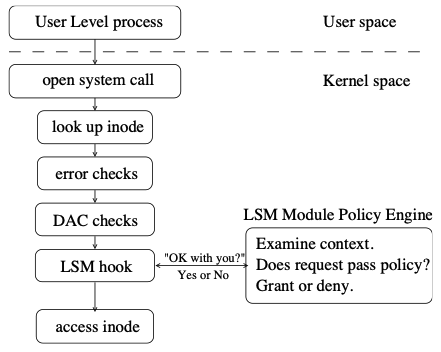
\includegraphics[width=0.6\linewidth]{lsm-hook-architecture.png}
  \caption{LSM Hook Architecture, from \cite{lsm-2002}.}
  \label{fig:lsm-hook-architecture}
\end{figure}

\subsection{Landlock}
\label{sec:intro-lsm-landlock}

\textit{Landlock} \cite{landlock-kernel, landlock-user-space} is a security feature available since Linux 5.13
that uses the LSM framework in order to provide scoped access control
so that any process, even when unprivileged, can securely restrict itself.
This can help mitigate the security impact of bugs or unexpected/malicious behaviour
in user space applications.

Landlock employs the concept of \textit{rule}, which describes an action
on an object. An object is (currently) a file hierarchy, and actions are
defined with access rights, such as executing, reading or writing files, making
symbolic links and so on.
A set of rules is called a \textit{ruleset}, and it can restrict both the thread
using it and its future children, created either by spawning a new thread, as well
as using the \textit{fork} system call.

Notably, Landlock does not permit the definition of exceptions.
For example, let us suppose we have a directory \texttt{dir1}, which contains two files
\texttt{file1} and \texttt{file2}. We can define a ruleset that allows
reading and writing files for \texttt{dir1}.
However, if we then define another ruleset comprising only of read operations
for \texttt{file1}, the permissions specified for \texttt{dir1} are still
valid, so when a process restricts itself it is still able to write to \texttt{file1}.

Other limitations of Landlock include the impossibility for a thread to modify its own topology
(e.g., via \textit{mount}), a limit of 16 layers of stacked rulesets and the impossibility to
restrict special file systems, such as kernel file systems (e.g., nsfs).

In case of multiple consecutive self-restrictions, the result is the intersection
of all rulesets - if a process first restricts itself allowing all read and writing operations,
and then restricts itself again with only reading permissions, the result is equivalent
to a single restriction made with a ruleset that permits only reading operations.

Landlock can be used directly when writing C/C++ code in Linux with the
\texttt{<linux/landlock.h>}\footnote{Examples of code available at \cite{landlock-user-space}.}
header, or by using libraries that provide these bindings to other languages,
such as \texttt{go-landlock} \cite{go-landlock}
for Go and \texttt{rust-landlock} \cite{rust-landlock} for Rust.

Landlock employs a series of flags to restrict a sandboxed process to a set of actions on files and
directories opened after the sandboxing operation (those opened before are not affected).
As highlighted in \cite{landlock-user-space}, the file system flags for files are:
\begin{itemize}
  \item \texttt{LANDLOCK\_ACCESS\_FS\_EXECUTE}, to execute a file;
  \item \texttt{LANDLOCK\_ACCESS\_FS\_WRITE\_FILE}, to open a file with write access;
  \item \texttt{LANDLOCK\_ACCESS\_FS\_READ\_FILE}, to open a file with read access.
\end{itemize}

Directories can receive a wider range of access rights, including the previous ones and the following ones.
All of them, except the first, are applied to the content of a directory and not to the directory
itself\footnote{This means that, for example, if \texttt{LANDLOCK\_ACCESS\_FS\_REMOVE\_DIR} is given to a directory $d$, it
allows the removal of empty directories \textit{inside} of $d$, and not of $d$ itself.}.
\begin{itemize}
  \item \texttt{LANDLOCK\_ACCESS\_FS\_READ\_DIR}, to open a directory or list its content\footnote{Applies to subdirectories as well.};
  \item \texttt{LANDLOCK\_ACCESS\_FS\_REMOVE\_DIR}, to remove an empty directory or rename one;
  \item \texttt{LANDLOCK\_ACCESS\_FS\_REMOVE\_FILE}, to unlink or rename a file;
  \item \texttt{LANDLOCK\_ACCESS\_FS\_MAKE\_CHAR}, to create, rename or link a character device;
  \item \texttt{LANDLOCK\_ACCESS\_FS\_MAKE\_DIR}, to create or rename a directory;
  \item \texttt{LANDLOCK\_ACCESS\_FS\_MAKE\_REG}, to create, rename or link a regular file;
  \item \texttt{LANDLOCK\_ACCESS\_FS\_MAKE\_SOCK}, to create, rename or link a socket;
  \item \texttt{LANDLOCK\_ACCESS\_FS\_MAKE\_FIFO}, to create, rename or link a named pipe;
  \item \texttt{LANDLOCK\_ACCESS\_FS\_MAKE\_BLOCK}, to create, rename or link a block device;
  \item \texttt{LANDLOCK\_ACCESS\_FS\_MAKE\_SYM}, to create, rename or link a symbolic link;
  \item \texttt{LANDLOCK\_ACCESS\_FS\_REFER}, to re-parent a file hierarchy\footnote{Available since the second version of the Landlock ABI.}.
\end{itemize}

This last one is treated differently from the others - in order to prevent privilege escalation,
it is necessary that the destination directory hierarchy has the same (or a superset of) restrictions
as the source hierarchy, since only create a rule with such access right is not enough to protect oneself.
If that is not the case, this actions is denied directly by the operating system.

Lastly, every new thread resulting from a \textit{clone} call inherits all Landlock restrictions from its parents.
These restrictions are also kept after a \textit{fork}.
More specifically, when a thread restricts itself, these rules are not applied to other sibling threads
but will be enforced on all of the thread's descendants.

\subsection{eBPF}
\textit{eBPF} \cite{ebpf} is a virtual machine in the Linux Kernel that can run sandboxed programs
in a privileged context. It can be used to safely extend the capabilities of the kernel
without requiring to change kernel source code or load kernel modules. A generic overview of its structure
is visible in Figure \ref{fig:ebpf-generic-overview}.

\begin{figure}[h]
  \centering
  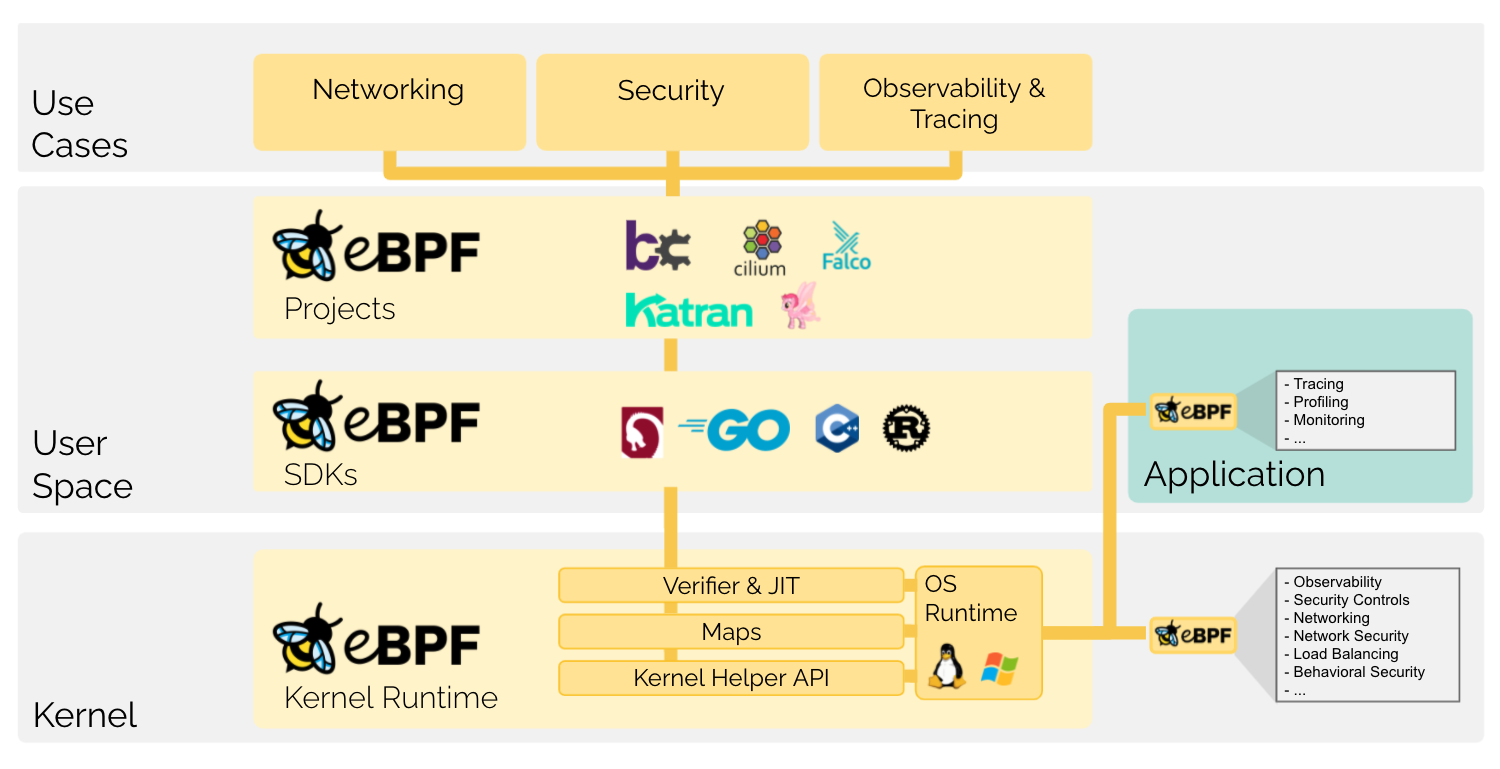
\includegraphics[width=0.8\linewidth]{ebpf-diagram.png}
  \caption{A generic overview of eBPF, from \cite{ebpf}.}
  \label{fig:ebpf-generic-overview}
\end{figure}

Some of the most common use cases for eBPF include the implementation of networking, security, and
observability of programs. These are usually implemented in the operating system because of the kernel's
privileges, but the kernel itself is hard to evolve.
On the other hand, application developers can run eBPF programs in order to add additional capabilities at runtime,
and then the operating system guarantees security and efficiency as if natively compiled
by using a Just-In-Time compiler.

These eBPF programs are event-driven and run when a certain hook point is passed. Some
predefined hooks include system calls, network events, and so on. If a hook does not exist,
it is possible to create custom kernel or user probes. An example of how eBPF interacts with the
Linux kernel is visible in Figure \ref{fig:example-ebpf-hooks}.

\begin{figure}[h]
  \centering
  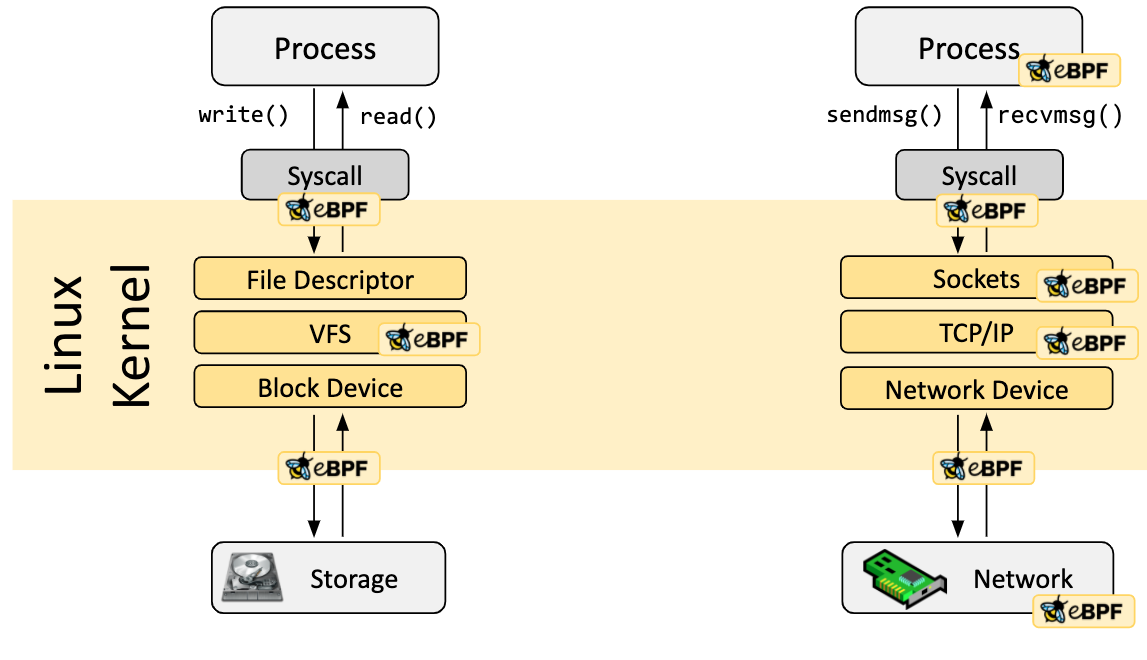
\includegraphics[width=0.8\linewidth]{ebpf-hooks.png}
  \caption{An example of two eBPF hooks, from \cite{ebpf-description}.}
  \label{fig:example-ebpf-hooks}
\end{figure}

When running a program with eBPF, there are many steps that are taken:
\begin{enumerate}
  \item first of all, eBPF is usually not used directly but via libraries that provide the ability to specify
        intent-based operations which are then implemented with eBPF; in any case, an eBPF program must be
        compiled into a specific eBPF bytecode;
  \item when a certain \textit{hook} is invoked, this hook has to be identified and then the program can be loaded
        into the kernel with a system call;
  \item a \textit{verification} step ensures that the eBPF program is safe to run by validating a set of conditions
        (e.g., the program has the required capabilities, the program always runs to completion, etc.);
  \item finally, the generic bytecode is then Just-In-Time \textit{compiled} into the machine instructions
        to run the program as efficiently as possible.
\end{enumerate}

Unlike Landlock, eBPF makes it possible to define specific exception, e.g., denying
certain access rights on specific files while allowing them on the containing directory.
It also allows to specify whether a program has access to devices such as \texttt{terminal}
and \texttt{dev}.
Thanks to \texttt{BPFContain} \cite{bpfcontain}
it is also possible to run a container security daemon by leveraging eBPF.  In this case,
specific policies must be written for desired commands.